\subsection{空对象模式}

空对象模式是一种用于替换空值的模式。它可以避免因操作空值而导致的空指针异常。

\begin{figure}[htb]
  \centering
  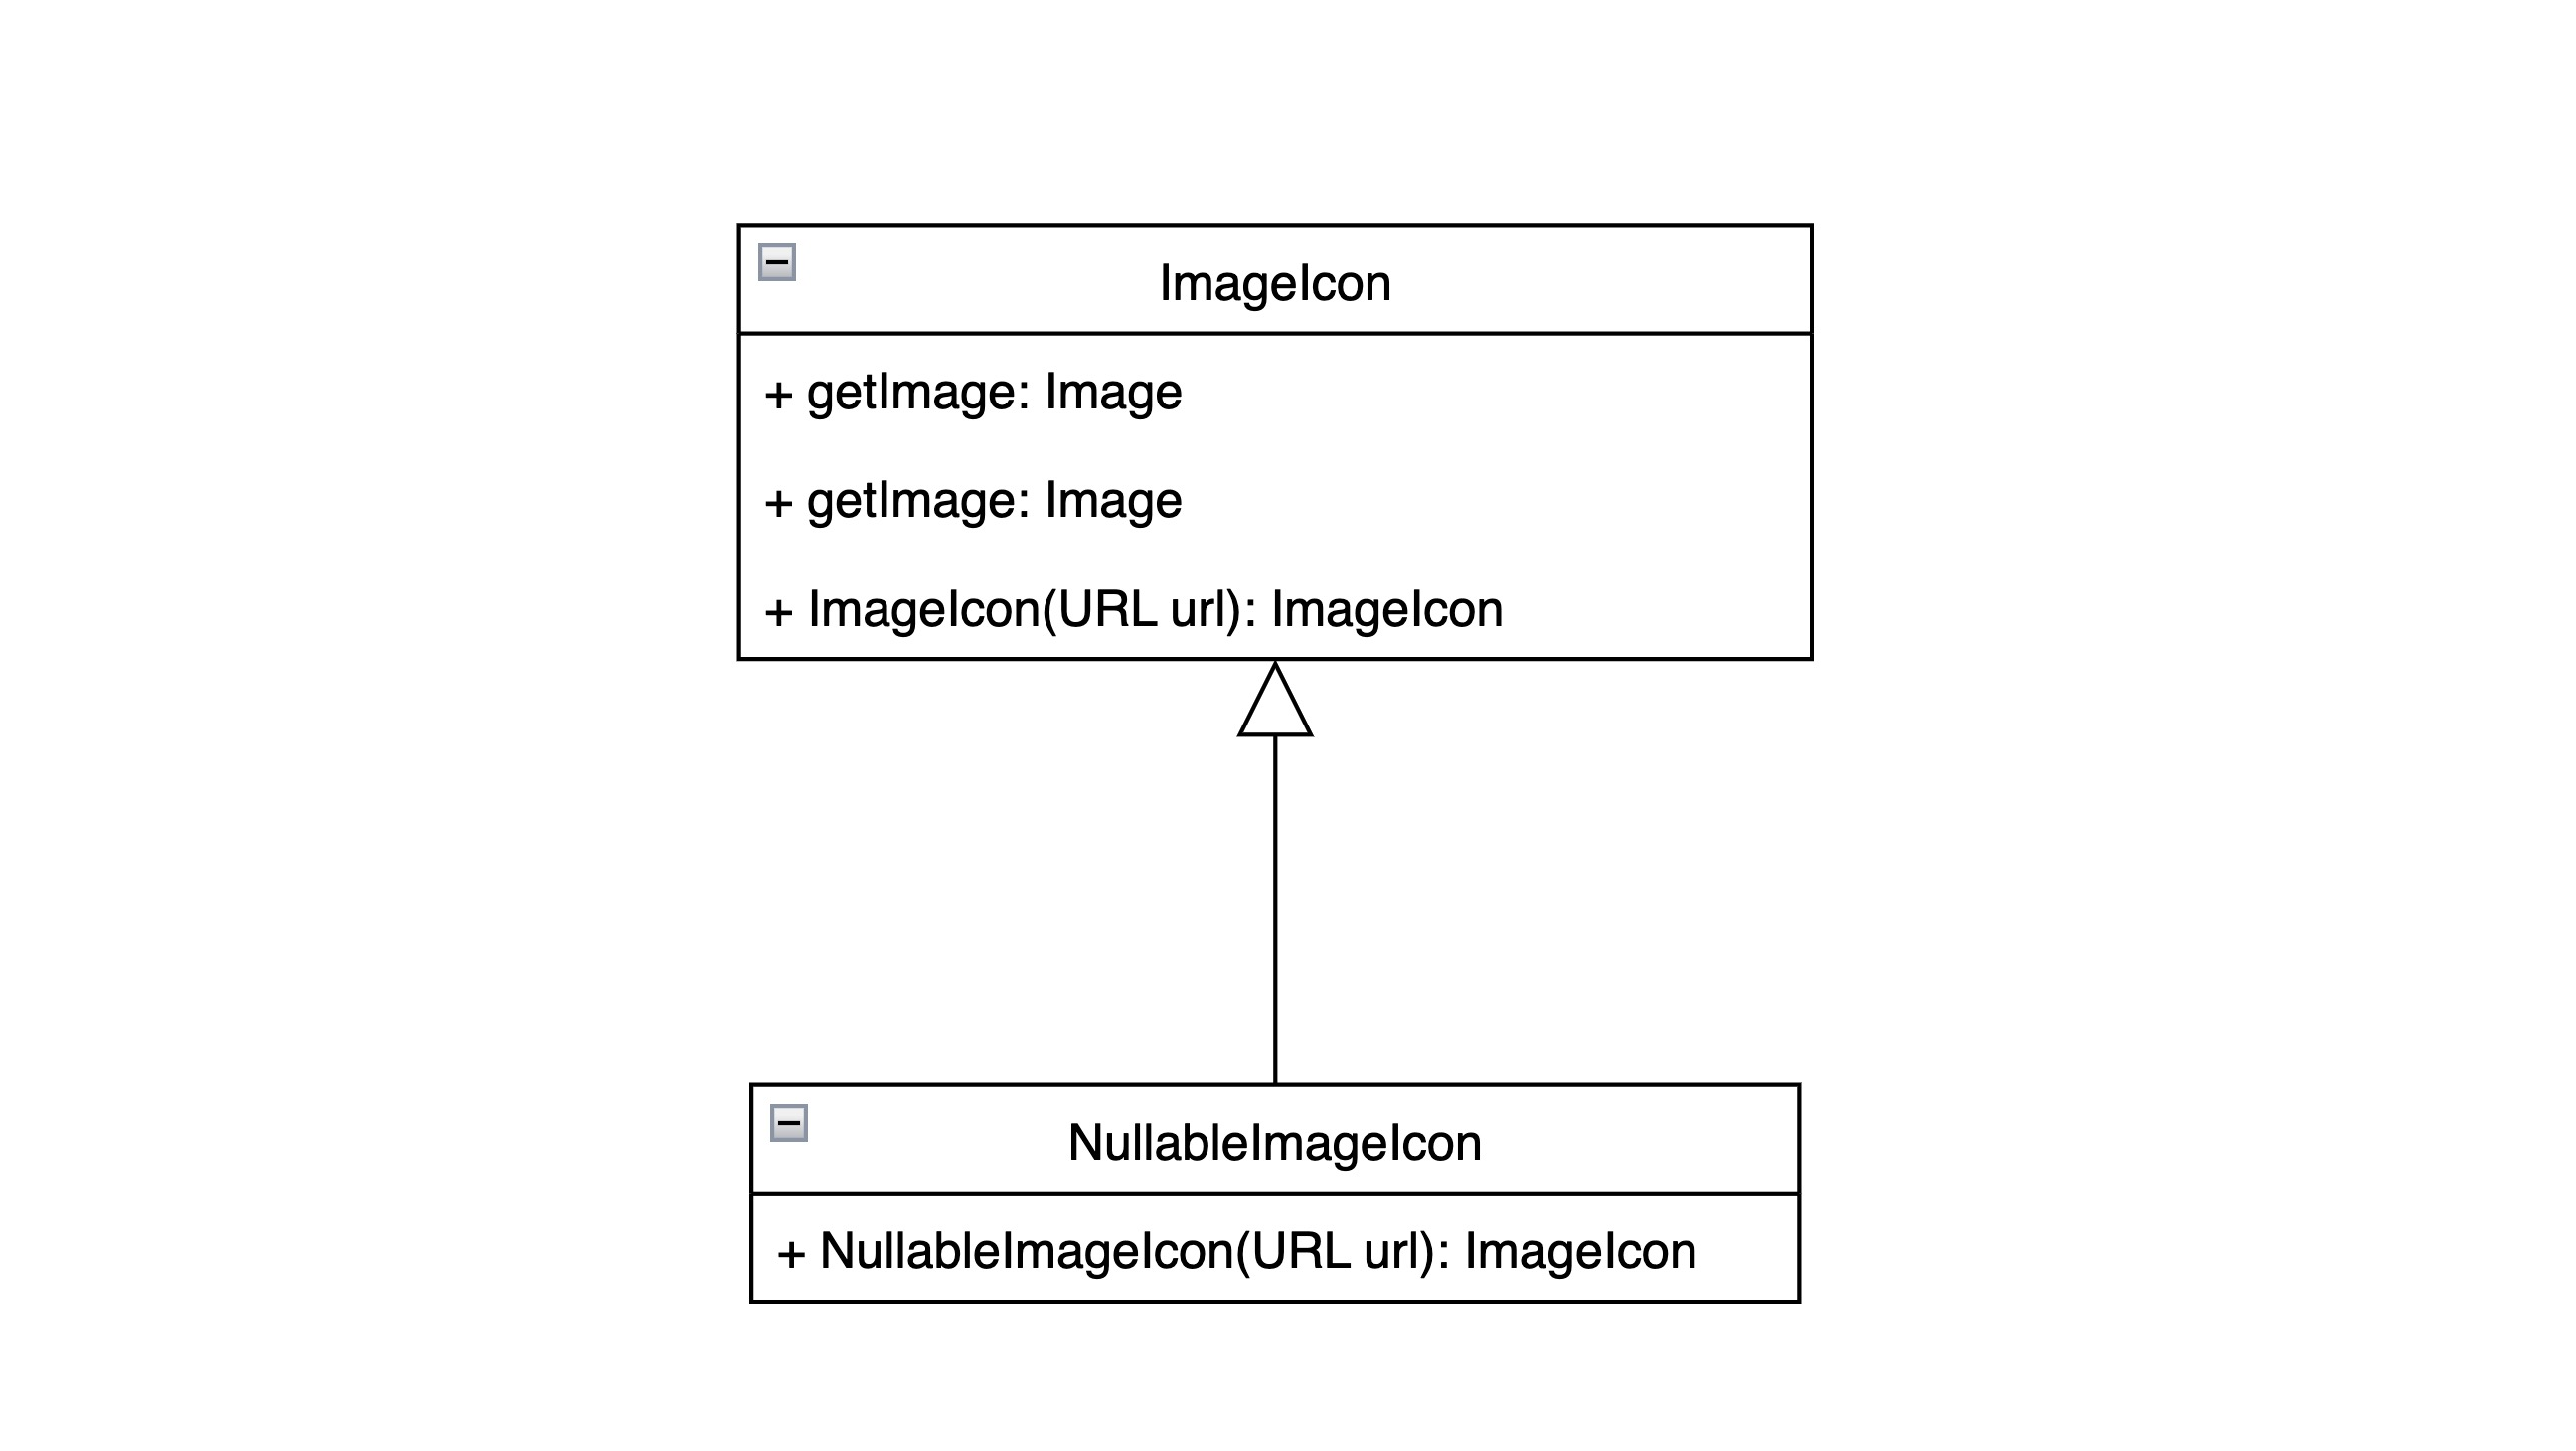
\includegraphics[width=0.9\textwidth]{figures/空对象模式.jpg}
  \caption{空对象模式在 Slow6502 中的类图}
\end{figure}

在StatusPanel组件中使用空对象模式,使得即使在没有资源文件图片存在的情况下,也可以正常显示图片组件,以默认图片作为空对象。

